\documentclass[10pt,a4paper]{article}
\usepackage[margin=22mm]{geometry}
\usepackage[T1]{fontenc}
\usepackage{lmodern,amsmath,amssymb,booktabs,graphicx,tikz,hyperref,fvextra}
\usetikzlibrary{arrows.meta,positioning,calc,decorations.pathmorphing}
\definecolor{ink}{RGB}{20,53,78}
\hypersetup{colorlinks=true,urlcolor=ink,linkcolor=ink}
\setlength{\parindent}{0pt}
\setlength{\parskip}{5pt}
\emergencystretch=3em

\title{\color{ink}A synthetic process from identification to validation}
\author{}
\date{Original learning collection -- November 2026}
\begin{document}
\begin{center}{\LARGE\color{ink}A synthetic process from identification to validation}\\[5pt]{\small Original learning collection -- November 2026}\end{center}

\textbf{Evidence note.} Original teaching scenario. Numerical parameters are deliberately chosen for learning. All generated data and curves are synthetic; no physical measurement is asserted.
\section{Design brief}
Create a reproducible synthetic identification experiment with gain $K=1.8$, time constant $\tau=4\,\mathrm{s}$ and delay $\theta=0.6\,\mathrm{s}$. Apply a two-unit step at $t=2\,\mathrm{s}$, sample every $0.05\,\mathrm{s}$ and add independent Gaussian noise with standard deviation $0.015$ using seed 2026. Estimate the parameters without initializing at truth, validate on a separate multistep record, and tune PI using $\lambda=2\,\mathrm{s}$. Assess the delayed closed loop with $u\in[0,2]$, distinguishing training, validation and simulated controller evaluation.
\section{Physical system}
\begin{center}\resizebox{\ifdim\width>.98\linewidth.98\linewidth\else\width\fi}{!}{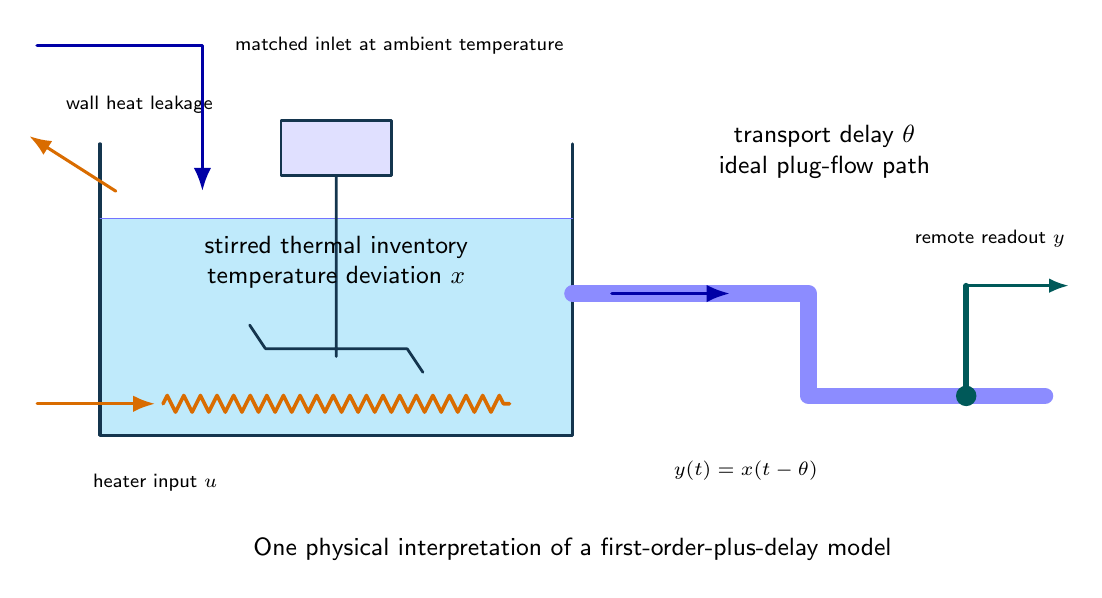
\begin{tikzpicture}[
font=\sffamily\small,>=Latex,line cap=round,line join=round,
wall/.style={draw=ink,line width=1.2pt,fill=blue!5},
water/.style={fill=cyan!25,draw=none},
metal/.style={draw=ink,fill=blue!12,line width=.9pt},
flow/.style={->,draw=blue!65!black,line width=1.2pt},
heat/.style={->,draw=orange!85!black,line width=1.1pt},
measure/.style={->,draw=teal!70!black,line width=.9pt},
dim/.style={<->,draw=ink!65,line width=.6pt},
spring/.style={draw=ink,decorate,decoration={coil,aspect=.5,segment length=4pt,amplitude=3pt}},
wire/.style={draw=ink,line width=1pt},
lab/.style={align=center,font=\sffamily\small},
smalllab/.style={align=center,font=\sffamily\scriptsize}]

\fill[water](1,.7)rectangle(7,3.45);
\draw[wall,fill=none](1,4.4)--(1,.7)--(7,.7)--(7,4.4);
\draw[blue!55](1,3.45)--(7,3.45);
\draw[metal](3.3,4)rectangle(4.7,4.7);
\draw[wire](4,4)--(4,1.7)(3.1,1.8)--(4.9,1.8)(3.1,1.8)--(2.9,2.1)(4.9,1.8)--(5.1,1.5);
\draw[orange!85!black,line width=1.3pt,decorate,decoration={zigzag,segment length=6pt,amplitude=3pt}](1.8,1.1)--(6.2,1.1);
\draw[heat](.2,1.1)--(1.7,1.1);
\node[smalllab]at(1.7,.1){heater input $u$};
\node[lab]at(4,2.9){stirred thermal inventory\\temperature deviation $x$};
\draw[heat](1.2,3.8)--(.1,4.5);
\node[smalllab]at(1.5,4.9){wall heat leakage};
\draw[flow](.2,5.65)--(2.3,5.65)--(2.3,3.8);
\node[smalllab]at(4.8,5.65){matched inlet at ambient temperature};
\draw[blue!45,line width=6pt](7,2.5)--(10,2.5)--(10,1.2)--(13,1.2);
\draw[flow](7.5,2.5)--(9,2.5);
\draw[teal!70!black,line width=2pt](12,1.2)--(12,2.6);
\fill[teal!70!black](12,1.2)circle(.13);
\draw[measure](12,2.6)--(13.3,2.6);
\node[smalllab]at(12.3,3.2){remote readout $y$};
\node[lab]at(10.2,4.3){transport delay $\theta$\\ideal plug-flow path};
\node[smalllab]at(9.2,.25){$y(t)=x(t-\theta)$};
\node[lab]at(7,-.75){One physical interpretation of a first-order-plus-delay model};
\end{tikzpicture}
}\par{\small A stirred thermal inventory followed by ideal transport is one possible physical interpretation of the identified transfer function. The effective conductance includes wall leakage and through-flow heat removal. Its fitted gain and time constant do not separately determine capacity, conductance and heater efficiency.}\end{center}
\section{A declared synthetic experiment}
The teaching plant is $G(s)=K e^{-\theta s}/(\tau s+1)$ with $K=1.8$, $\tau=4$ s and $\theta=0.6$ s. These values define a simulation, not measured equipment. For an input step of amplitude $A$ at $t_0$,
\[y(t)=KA\left(1-e^{-(t-t_0-\theta)/\tau}\right)\mathbf1_{t\ge t_0+\theta}.\]
Independent Gaussian noise is added with a stated seed. The optimizer receives bounds and the starting guess $(1,2,0.2)$, not the true parameters.
\section{Identification and a separate check}
Minimize the sum of squared residuals between the noisy training samples and the delayed-step expression. Use positive bounds on gain and time constant and a nonnegative delay. Then form an independent multistep response by superposing signed step increments. Do not refit on this validation record.
Report training and validation RMSE. A good fit on both synthetic records checks the computation under the chosen model class; it does not establish that a real plant follows that class or quantify experimental uncertainty.
\section{Controller calculation}
With estimated parameters $\hat K,\hat\tau,\hat\theta$ and chosen $\lambda=2$ s, use the standard IMC-style PI tuning rule
\[K_p=\frac{\hat\tau}{\hat K(\lambda+\hat\theta)},\qquad K_i=K_p/\hat\tau.\]
This is the standard \href{https://apmonitor.com/pdc/index.php/Main/ProportionalIntegralControl}{APMonitor IMC-style PI tuning rule}. Evaluate the controller against the declared true synthetic plant, including its pure input delay and actuator limit.
\section{Delay implementation and limitations}
Use a 0.01 s numerical control interval. The true delay is exactly 60 such intervals, so a history buffer applies the delayed held input without a Pade approximation. Propagate the first-order plant with its exact held-input update. Add a constant output-equivalent process disturbance after 15 s and use integral back-calculation when the actuator clips.
This evaluation has numerical sampling, exact nominal plant parameters and noiseless feedback. It is not a hardware test, robustness proof, statistical confidence interval or validation against independent real measurements.
\section{What to learn from the experiment}
Training, validation and controller evaluation answer different questions. All three records are synthetic here; experimental claims require independently collected measurements.
\section{System sketch}
\begin{center}\resizebox{\ifdim\width>.98\linewidth.98\linewidth\else\width\fi}{!}{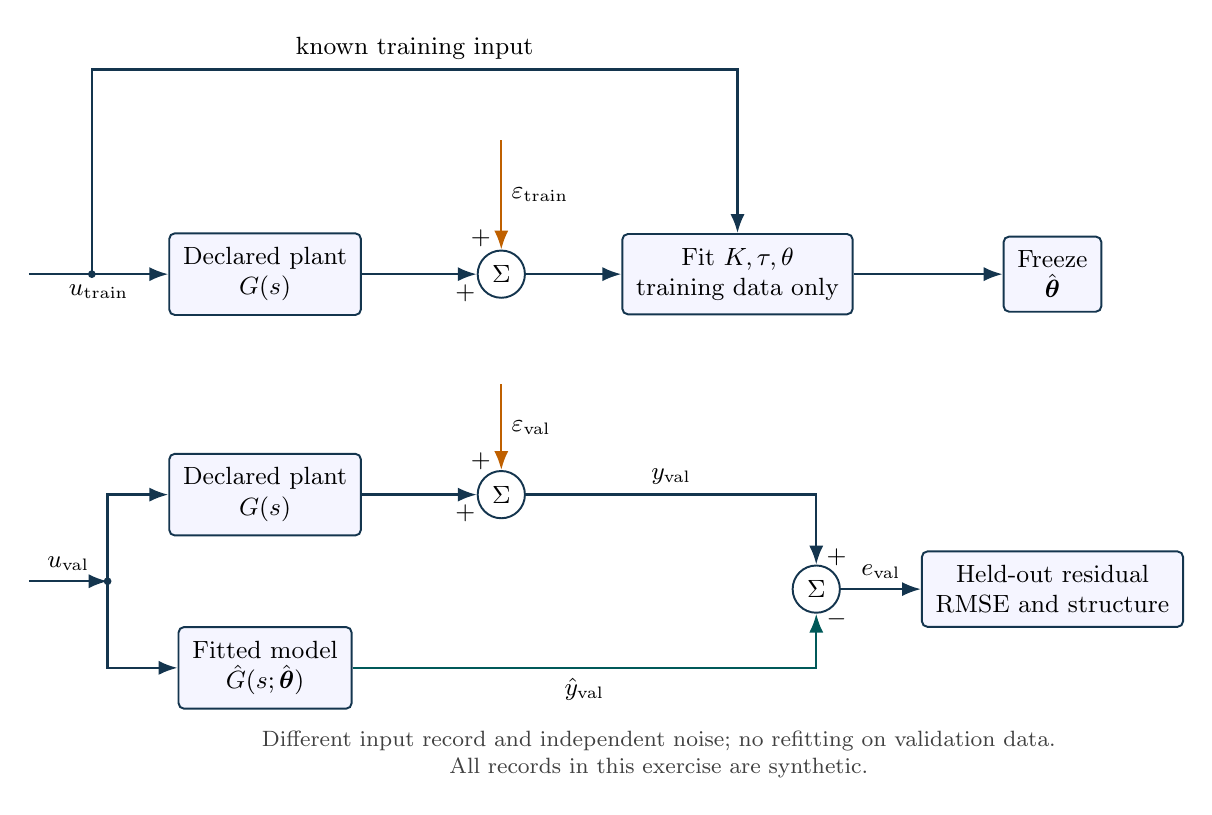
\begin{tikzpicture}[x=1cm,y=1cm,>=Latex,font=\small,
block/.style={draw=ink,fill=blue!4,rounded corners=2pt,minimum height=9mm,align=center,line width=.7pt,inner sep=5pt},
sum/.style={circle,draw=ink,fill=white,minimum size=6mm,inner sep=0pt,line width=.7pt},
sig/.style={->,draw=ink,line width=.85pt},
fb/.style={->,draw=teal!70!black,line width=.85pt},
dist/.style={->,draw=orange!75!black,line width=.85pt},
tap/.style={circle,fill=ink,inner sep=1.4pt},
note/.style={font=\footnotesize,align=center,text=black!75}]

\node[block](plant)at(3,1.5){Declared plant\\$G(s)$};
\node[sum](noise)at(6,1.5){$\Sigma$};
\node[block](fit)at(9,1.5){Fit $K,\tau,\theta$\\training data only};
\node[block](freeze)at(13,1.5){Freeze\\$\hat{\boldsymbol\theta}$};
\draw[sig](0,1.5)--node[below]{$u_{\mathrm{train}}$}(plant);
\draw[sig](plant)--node[pos=.9,below]{$+$}(noise);
\draw[dist](6,3.2)--node[right]{$\varepsilon_{\mathrm{train}}$}node[pos=.9,left]{$+$}(noise);
\draw[sig](noise)--(fit);\draw[sig](fit)--(freeze);
\draw[sig](.8,1.5)--(.8,4.1)--node[above]{known training input}(9,4.1)--(fit.north);
\fill[ink](.8,1.5)circle(1.4pt);
\node[block](truth)at(3,-1.3){Declared plant\\$G(s)$};
\node[block](pred)at(3,-3.5){Fitted model\\$\hat G(s;\hat{\boldsymbol\theta})$};
\node[sum](nv)at(6,-1.3){$\Sigma$};
\node[sum](err)at(10,-2.5){$\Sigma$};
\node[block](metric)at(13,-2.5){Held-out residual\\RMSE and structure};
\draw[sig](0,-2.4)--node[above]{$u_{\mathrm{val}}$}(1,-2.4);
\draw[sig](1,-2.4)--(1,-1.3)--(truth);
\draw[sig](1,-2.4)--(1,-3.5)--(pred);
\fill[ink](1,-2.4)circle(1.4pt);
\draw[sig](truth)--node[pos=.9,below]{$+$}(nv);
\draw[dist](6,.1)--node[right]{$\varepsilon_{\mathrm{val}}$}node[pos=.9,left]{$+$}(nv);
\draw[sig](nv)--node[above]{$y_{\mathrm{val}}$}(10,-1.3)--node[pos=.9,right]{$+$}(err);
\draw[fb](pred)--node[below]{$\hat y_{\mathrm{val}}$}(10,-3.5)--node[pos=.9,right]{$-$}(err);
\draw[sig](err)--node[above]{$e_{\mathrm{val}}$}(metric);
\node[note]at(8,-4.6){Different input record and independent noise; no refitting on validation data.\\All records in this exercise are synthetic.};

\end{tikzpicture}
}
\par\small\refstepcounter{figure}\label{fig:system}\textbf{Figure \thefigure.} Training selects parameters; held-out validation freezes them. Separate noise records avoid reusing training residuals as validation evidence.\end{center}
\newpage
\section{Executed computational evidence}
\VerbatimInput[fontsize=\small,breaklines=true]{results.txt}
\begin{center}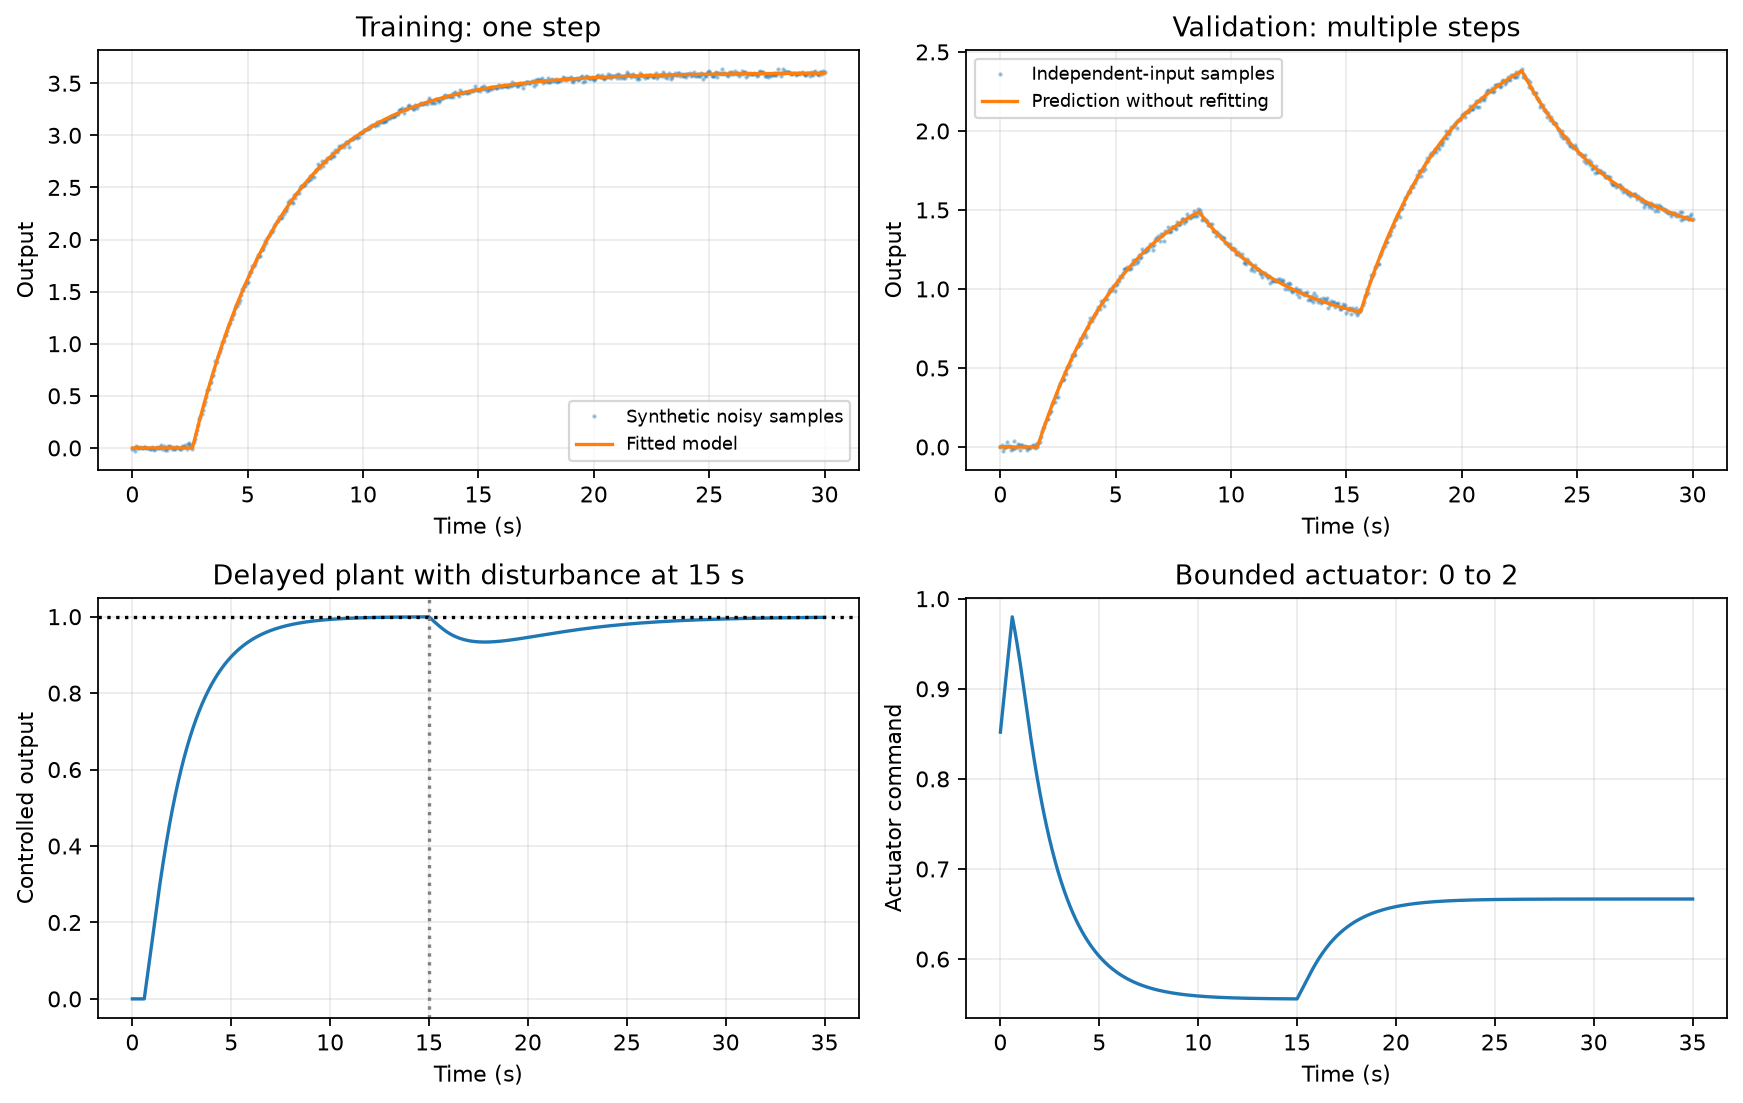
\includegraphics[width=\linewidth,height=.39\textheight,keepaspectratio]{response.png}\end{center}
\textbf{Reading the panels.} The upper row compares the training fit with prediction on a separate synthetic input record. The lower row shows the simulated closed-loop disturbance response and constrained actuator command. These are numerical checks under the declared model, not measurements of a physical process.
\end{document}
